\documentclass[tikz,border=6pt]{standalone}
\usepackage{xcolor}
\usetikzlibrary{arrows.meta,positioning}

\definecolor{blockblue}{HTML}{4A90D9}
\definecolor{linegray}{HTML}{333333}
\definecolor{sumgreen}{HTML}{5CB85C}

\begin{document}
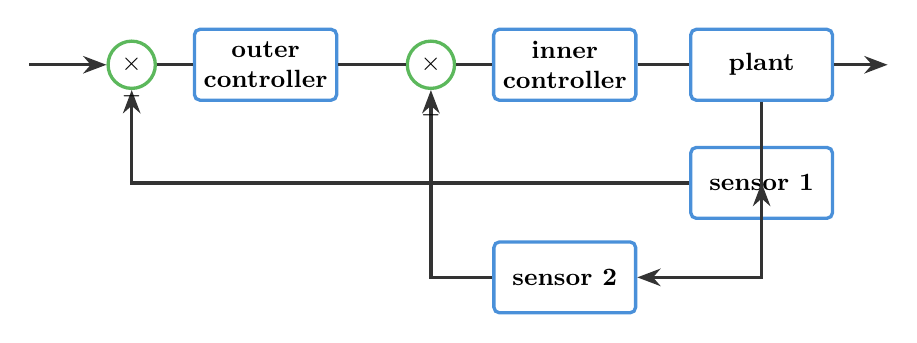
\begin{tikzpicture}[
  >=Stealth,
  line width=1.2pt,
  block/.style={rectangle, draw=blockblue, rounded corners=2pt, minimum width=1.8cm, minimum height=0.9cm, align=center, font=\small\bfseries},
  flow/.style={->, draw=linegray, line width=1.2pt},
  sum/.style={circle, draw=sumgreen, minimum size=6mm, inner sep=0pt}
]
  \node[sum] (s1) at (0.8,0) {}; \node at (0.8,0) {\small $\times$};
  \node[block] (c1) at (2.5,0) {outer\\controller};
  \node[sum] (s2) at (4.6,0) {}; \node at (4.6,0) {\small $\times$};
  \node[block] (c2) at (6.3,0) {inner\\controller};
  \node[block] (p) at (8.8,0) {plant};
  \node[block] (sen1) at (8.8,-1.5) {sensor 1};
  \node[block] (sen2) at (6.3,-2.7) {sensor 2};
  \draw[flow] (-0.5,0) -- (s1);
  \draw[flow] (s1) -- (c1) -- (s2) -- (c2) -- (p) -- (10.4,0);
  \draw[flow] (p) |- (sen1);
  \draw[flow] (sen1) -| node[pos=0.86, above, font=\small] {$-$} (s1);
  \draw[flow] (p) |- (sen2);
  \draw[flow] (sen2) -| node[pos=0.88, above, font=\small] {$-$} (s2);
\end{tikzpicture}
\end{document}
